\begin{exercise}
Implementieren Sie das implizite Euler-Verfahren unter Verwendung des Newton-Verfahrens
zur Lösung des nichtlinearen Gleichungssystems. Der Algorithmus soll als Input-Parameter
einen Vektor von Stützstellen $t$, einen Startwert $y_0$, die rechte Seite und Ableitung
der rechten Seite $f$, beziehungsweise $\frac{\partial}{\partial y} f$, sowie eine
geeignete Abbruchbedingung für das Newton-Verfahren (Toleranz und/oder maximale
Anzahl an Iterationen) akzeptieren. \\
Testen Sie das Verfahren an folgenden Anfangswertproblemen: Sei $Y = (y_1,y_2)^{\top}$
die Lösung des Anfangswertproblems
\begin{align}
  Y^{\prime}(t) = \begin{pmatrix}
    -2 & 1 \\
    1 & -2
  \end{pmatrix}Y(t) +
  \begin{pmatrix}
    2 \sin(t) \\ 2(\cos(t) - \sin(t))
  \end{pmatrix},\quad t \geq 0, \qquad
  Y(0) = \begin{pmatrix}
    2 \\ 3
  \end{pmatrix}.
\end{align}
Sei $Z = (z_1,z_2)^{\top}$ die Lösung des Anfangswertproblems
\begin{align}
Z^{\prime}(t) = \begin{pmatrix}
  -2 & 1 \\ 998 & -999
\end{pmatrix}Z(t) +
\begin{pmatrix}
  2\sin(t) \\ 999(\cos(t)-\sin(t))
\end{pmatrix}, \quad t \geq 0, \qquad
Z(0) = \begin{pmatrix}
  2 \\ 3
\end{pmatrix}.
\end{align}
Vergleichen Sie dabei auch mit den Ergebnissen und Schrittweiten des eingebetteten
Runge-Kutta-Verfahren RK5(4) aus Aufgabe 15. Verwenden Sie dazu die Parameter $t \in
[0,10], \rho = 0.7, \eta = 1.5,$ tol$=10^{-6}, h_{\min} = 10^{-10}$.
\end{exercise}
\begin{solution}
Wir beobachten, dass beide Differentialgleichungen zu annähernd gleichen Ergebnissen
führen, im zweiten Fall werden allerdings im eingebetteten Runge-Kutta-Verfahren
deutlich kleinere Schrittweiten für die selbe Genauigkeit benötigt.
\FloatBarrier
\begin{figure}
    \centering
    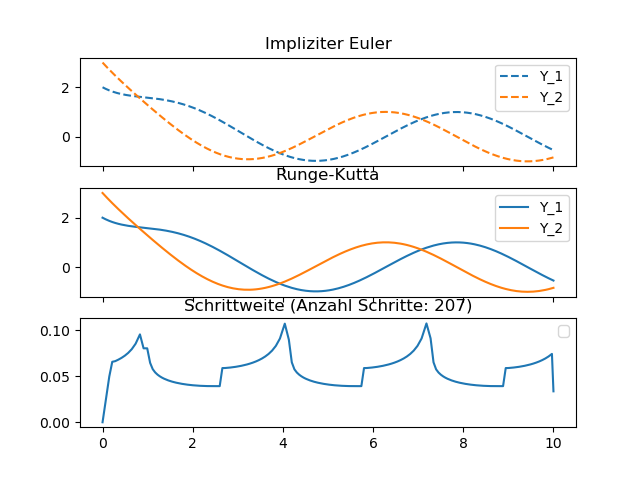
\includegraphics[width=\linewidth]{plot1_advanced.png}
    \caption{Y}
\end{figure}
\begin{figure}
    \centering
    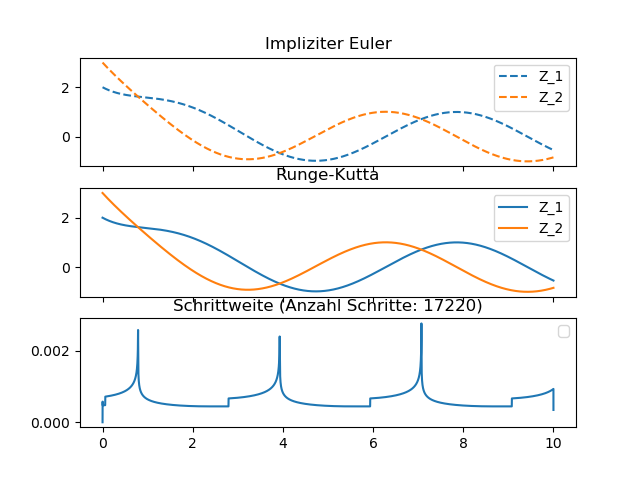
\includegraphics[width=\linewidth]{plot2_advanced.png}
    \caption{Z}
\end{figure}
\end{solution}
